\documentclass[10pt]{beamer}
\usepackage[utf8]{inputenc}
\usepackage[T1]{fontenc}
\usepackage[english]{babel}
\usepackage{amssymb,amsthm,amsmath,amsfonts}
\usepackage{lmodern}
\usepackage{tikz}

\usetheme{Boadilla}

\setbeamertemplate{footline}{%
  \leavevmode%
  \hbox{\begin{beamercolorbox}[wd=.5\paperwidth,ht=2.5ex,dp=1.125ex,leftskip=.3cm plus1fill,rightskip=.3cm]{author in head/foot}%
    \usebeamerfont{author in head/foot}\insertshortauthor
  \end{beamercolorbox}%
  \begin{beamercolorbox}[wd=.5\paperwidth,ht=2.5ex,dp=1.125ex,leftskip=.3cm,rightskip=.3cm plus1fil]{title in head/foot}%
    \usebeamerfont{title in head/foot}\insertshorttitle \hfill
    \insertframenumber/\inserttotalframenumber
  \end{beamercolorbox}}%
  \vskip0pt%
}
\definecolor{pacificcream}{cmyk}{.05,.05,.15,0}

\beamertemplatenavigationsymbolsempty

\theoremstyle{plain}
\newtheorem{thm}{Theorem}[part]
\theoremstyle{definition} 
\newtheorem{lem}[thm]{Lemma}
\theoremstyle{definition} 
\newtheorem{cor}[thm]{Corollary}
\theoremstyle{definition} 
\newtheorem{prop}[thm]{Proposition}
\theoremstyle{definition} 
\newtheorem{defi}[thm]{Definition}
\theoremstyle{remark} 
\newtheorem{rem}[thm]{Remark}
\theoremstyle{remark} 
\newtheorem{exe}[thm]{Example}

\newcommand{\orangebox}[2]{\begin{block}{#1}#2\end{block}}
\renewcommand{\emph}[1]{{\usebeamercolor[fg]{structure}#1}}

\def\C{\mathbb{C}}
\def\Z{\mathbb{Z}}
\def\F{\mathbb{F}}

\def\red#1{\textcolor{red}{#1}}
\def\blu#1{\textcolor{blue}{#1}}

\tikzset{position/.style args={#1:#2 from #3}{%
  at=(#3.#1),anchor=#1+180,shift=(#1:#2)}}%
\tikzstyle{lambda}=[very thick,draw=blue,->]
\tikzstyle{mu}=[very thick,draw=red,->]

\usetikzlibrary{matrix,decorations,decorations.text,calc}

\pgfkeys{/triangle/.code=\tikzset{x={(-0.5cm,-0.866cm)},y={(1cm,0cm)}}}
\pgfkeys{/lattice/.code n args={4}{\tikzset{cm={#1,#2,#3,#4,(0,0)}}}}

\newcommand{\axes}[4]{
  \clip (#1,#3) rectangle (#2,#4);
  \draw [thin, gray, -latex] (#1,0) -- (#2,0);% Draw x axis
  \draw [thin, gray, -latex] (0,#3) -- (0,#4);% Draw y axis
}

\newcommand{\lattice}[2]{
  \draw[style=help lines,dashed] (#1-1,#1-1) grid[step=1] (#2+1,#2+1);
  \foreach \x in {#1,...,#2}{
    \foreach \y in {#1,...,#2}{
      \node[draw,circle,inner sep=2pt,fill] at (\x,\y) {};
      % Places a dot at those points
    }
  }
}


\begin{document}

\author[Luca De Feo]{Luca De Feo\\
  \small joint work with Cyril Hugounenq, Jérôme Plût, Éric Schost}
\title{Explicit isogenies in quadratic time in any characteristic} 
\institute{Université de Neuchâtel}
\date{September 28, 2016}


\begin{frame}
\titlepage

\begin{center}
  \includegraphics[height=10mm]{Images/uvsq-logo-cmjn.jpg}  
\end{center}
\end{frame}


%%%%%%%%%%%%%%%%%%%%%%%%%%%%%%%%%%%%%%%%%%%%%%%%%%%%%%%%%%%%
%%%%%%%%%%%%%%%%%%%%%%%%%%%%%%%%%%%%%%%%%%%%%%%%%%%%%%%%%%%%

\section{Isogenies}

\begin{frame}
  \frametitle{Elliptic curves}

  Let $E$ be an elliptic curve\dots \uncover<2->{forget it!}

  \begin{center}
    \begin{tikzpicture}[domain=-2.4566:4,samples=100,yscale=1/2.2]
      \draw plot (\x,{sqrt(\x*\x*\x-4*\x+5)});
      \draw plot (\x,{-sqrt(\x*\x*\x-4*\x+5)});

      \draw[thin,gray,-latex] (0,-7) -- (0,7);
      \draw[thin,gray,-latex] (-3,0) -- (4,0);

      \draw (-3,1) -- (4,8/3+3);
      \begin{scope}[every node/.style={draw,circle,inner sep=1pt,fill},cm={1,2/3,0,0,(0,3)}]
        \node at (-2.287980,0) {};
        \node at (-0.535051,0) {};
        \node at (3.267475,0) {};
      \end{scope}
      \begin{scope}[every node/.style={yshift=0.3cm},cm={1,2/3,0,0,(0,3)}]
        \node at (-2.287980,0) {$P$};
        \node at (-0.535051,0) {$Q$};
        \node at (3.267475,0) {$R$};
      \end{scope}

      \draw[dashed] (3.267475,3.267475*2/3+3) -- (3.267475,-3.267475*2/3-3) 
      node[draw,circle,inner sep=1pt,fill] {}
      node[xshift=-0.1cm,anchor=east] {$P+Q$};

      \begin{uncoverenv}<2>
        \draw[very thick,red] (-5,-7) -- (6,7);
        \draw[very thick,red] (-5,7) -- (6,-7);
      \end{uncoverenv}
    \end{tikzpicture}
  \end{center}
\end{frame}

%%

\begin{frame}
  \frametitle{Elliptic curves}

  \begin{columns}
    \begin{column}{0.75\textwidth}
      \begin{tikzpicture}[scale=2]
        \axes{-1}{3.5}{-0.5}{3}

        \begin{scope}[/lattice={1}{0.2}{0.4}{0.7}]
          \begin{uncoverenv}<1>
            \draw[fill,black!10] (0,0) -- (1,0) -- (1,1) -- (0,1) -- (0,0);
            \node at (0.5,0.5) {$\C/\Lambda$};
            \node at (0.9,-0.1) {$\omega_1$};
            \node at (-0.1,0.9) {$\omega_2$};
          \end{uncoverenv}

          \lattice{-3}{4}

          \begin{uncoverenv}<2-5>
            \node[red] at (0.7,0.65) {$a$}; 
            \node[draw,circle,inner sep=1pt,fill,red] at (0.8,0.5) {};
            \node[red] at (0.2,0.9) {$b$}; 
            \node[draw,circle,inner sep=1pt,fill,red] at (0.3,0.7) {};
            
            \begin{uncoverenv}<3-4>
              \node[red] at (1.2,1.3) {$a+b$}; 
              \node[draw,circle,inner sep=1pt,fill,red] at (1.1,1.2) {};
              \begin{uncoverenv}<3>
                \draw[red,thin] (0,0) -- (0.8,0.5) -- (1.1,1.2);
                \draw[red,thin] (0,0) -- (0.3,0.7) -- (1.1,1.2);          
              \end{uncoverenv}
            \end{uncoverenv}

            \transdissolve<5>
            \begin{uncoverenv}<5>
              \node[red] at (0.2,0.3) {$a+b$}; 
              \node[draw,circle,inner sep=1pt,fill,red] at (0.1,0.2) {};
            \end{uncoverenv}
          \end{uncoverenv}
        \end{scope}  
      \end{tikzpicture}
    \end{column}
    \begin{column}{0.2\textwidth}
      \begin{onlyenv}<1>
        Let $\omega_1,\omega_2\in\C$ be linearly independent complex
        numbers. Set
        \[\emph{\Lambda = \omega_1\Z \oplus \omega_2\Z}\]

        $\C/\Lambda$ is an elliptic curve.
      \end{onlyenv}

      \begin{onlyenv}<2->
        Addition law induced by addition on $\C$.
      \end{onlyenv}
    \end{column}
  \end{columns}
\end{frame}

%%

\begin{frame}
  \frametitle{Isomorphism classes}

  \begin{columns}
    \begin{column}{0.7\textwidth}
      \begin{tikzpicture}[scale=2]
        \axes{-1}{3.3}{-0.5}{3}

        \newcount\scale
        \animate<1-21>
        \animatevalue<1-21>{\scale}{0}{20}
        \begin{uncoverenv}<1-22>
          \begin{scope}[/lattice={1}{0.2}{0.4}{0.7},scale=1+\the\scale/20,rotate=\the\scale]
            \lattice{-3}{4}
            \node[red,yshift=0.2cm] at (0.8,0.5) {$a$}; 
            \node[draw,circle,inner sep=1pt,fill,red] at (0.8,0.5) {};
          \end{scope}
        \end{uncoverenv}
      \end{tikzpicture}      
    \end{column}
    \begin{column}{0.25\textwidth}
      Two lattices are \emph{homotetic} if there exist $\alpha\in\C$
      such that
      \[\emph{\alpha\Lambda_1 = \Lambda_2}\]

      The \alert{$j$-invariant} $j(\Lambda)$ classifies elliptic curves
      up to \emph{homothety} (\emph{isomorphism}).
    \end{column}
  \end{columns}
\end{frame}  

%%

\begin{frame}
  \frametitle{Multiplication}

  \begin{tikzpicture}[scale=2.2]
    \axes{-1}{4.5}{-0.5}{3}

    \begin{scope}[/lattice={1}{0.2}{0.4}{0.7}]
      \lattice{-3}{5}
    
      \node[red,yshift=0.2cm] at (0.8,0.6) {$a$}; 
      \draw[red] (0.8,0.6) node[fill,circle,inner sep=1pt] {};

      \begin{uncoverenv}<2>
        \node[red,yshift=0.2cm] at (2.4,1.8) {$[3]a$}; 
        \draw[red] (0,0) -- (1.6,1.2) node[fill,circle,inner sep=1pt] {} 
        -- (2.4,1.8) node[fill,circle,inner sep=1pt] {};
      \end{uncoverenv}

      \transdissolve<3>
      \begin{uncoverenv}<3>
        \node[red,yshift=0.3cm] at (0.4,0.8) {$[3]a$}; 
        \draw[red] (0.4,0.8) node[fill,circle,inner sep=1pt] {};
      \end{uncoverenv}
    \end{scope}
  \end{tikzpicture}
\end{frame}

%%

\begin{frame}
  \frametitle{Multiplication + homothety}

  \begin{tikzpicture}[scale=2.2]
    \axes{-1}{4.5}{-0.5}{3}

    \begin{scope}[/lattice={3}{0.6}{1.2}{2.1}]
      \begin{uncoverenv}<1-2>
        \node[red,yshift=0.3cm] at (0.8,0.6) {$\uncover<2>{[3]}a$}; 
        \draw[red] (0.8,0.6) node[fill,circle,inner sep=1pt] {};
      \end{uncoverenv}

      \uncover<1>{\lattice{-1}{2}}
    \end{scope}
    
    \begin{scope}[/lattice={1}{0.2}{0.4}{0.7}]
      \transdissolve<2>
      \uncover<2->{\lattice{-3}{5}}

      \transdissolve<3>
      \begin{uncoverenv}<3>
        \node[red,yshift=0.3cm] at (0.4,0.8) {$[3]a$}; 
        \draw[red] (0.4,0.8) node[fill,circle,inner sep=1pt] {};
      \end{uncoverenv}
    \end{scope}
  \end{tikzpicture}  
\end{frame}

%%

\begin{frame}
  \frametitle{Torsion subgroups}

  \begin{columns}
    \begin{column}{0.7\textwidth}
      \begin{tikzpicture}[scale=1.8]
        \axes{-0.3}{4.5}{-0.5}{4};

        \begin{scope}[/lattice={3}{0.6}{1.2}{2.1}]
          \lattice{-1}{2}

          \foreach \i in {0,...,2} {
            \foreach \j in {0,...,2} {
              \draw[red] (\i/3,\j/3) node[fill,circle,inner sep=1pt] {};
            }
          }
          \draw[red] (0,0) -- (1/3,0) node[yshift=0.2cm] {$a$};
          \draw[red] (0,0) -- (0,1/3) node[yshift=0.2cm] {$b$};
        \end{scope}
      \end{tikzpicture}  
    \end{column}
    \begin{column}{0.25\textwidth}
      The $\ell$-torsion subgroup is made up by the points
      \[\emph{\left(\frac{i\omega_1}{\ell},\frac{j\omega_2}{\ell}\right)}\]

      It is a group of rank two
      \begin{alertenv}
        \begin{align*}
          E[\ell] &= \langle a,b \rangle\\
          &\simeq (\Z/\ell\Z)^2
        \end{align*}
      \end{alertenv}
    \end{column}
  \end{columns}
\end{frame}

%%

\begin{frame}
  \frametitle{Isogenies}

  \begin{columns}
    \begin{column}{0.7\textwidth}
      \begin{tikzpicture}[scale=1.8]
        \axes{-0.3}{4.5}{-0.5}{4};
        
        \begin{scope}[/lattice={3}{0.6}{1.2}{2.1}]
          \uncover<1>{\lattice{-1}{2}}

          \begin{uncoverenv}<1-3>
            \draw[red] (0,0) -- (1/3,0) node[yshift=0.3cm] {$a$};
          \end{uncoverenv}
          \begin{uncoverenv}<4->
            \draw[red] (0,0) -- (0,1/3) node[yshift=0.3cm] {$b$};
          \end{uncoverenv}

          \begin{uncoverenv}<1-2>
            \draw[blue] (0.8,0.5) node[yshift=0.3cm] {$p$};
            \draw[blue] (0.8,0.5) node[fill,circle,inner sep=1pt] {};
          \end{uncoverenv}
        \end{scope}
        
        \begin{scope}[/lattice={1}{0.2}{1.2}{2.1}]
          \transdissolve<2>
          \uncover<2-4>{\lattice{-3}{5}}

          \transdissolve<3>
          \begin{uncoverenv}<3-5>
            \draw[blue] (0.4,0.5) node[yshift=0.3cm] {$p$};
            \draw[blue] (0.4,0.5) node[fill,circle,inner sep=1pt] {};
          \end{uncoverenv}
        \end{scope}

        \begin{scope}[/lattice={1}{0.2}{0.4}{0.7}]
          \transdissolve<5>
          \uncover<5->{\lattice{-3}{5}}

          \transdissolve<6>
          \begin{uncoverenv}<6->
            \draw[blue] (0.4,0.5) node[yshift=0.3cm] {$p$};
            \draw[blue] (0.4,0.5) node[fill,circle,inner sep=1pt] {};
          \end{uncoverenv}
        \end{scope}
        
        \begin{scope}[/lattice={3}{0.6}{1.2}{2.1}]
          \foreach \i in {0,...,2} {
            \foreach \j in {0,...,2} {
              \draw[red] (\i/3,\j/3) node[fill,circle,inner sep=1pt] {};
            }
          }
        \end{scope}
      \end{tikzpicture}  
    \end{column}
    \begin{column}{0.25\textwidth}
      \begin{onlyenv}<1-3>
        Let $\red{a}\in\C/\Lambda_1$ be an $\ell$-torsion point, and let
        \[\emph{\Lambda_2 = a\Z\oplus\Lambda_1}\]
        Then \emph{$\Lambda_1\subset\Lambda_2$} and we define a degree
        $\ell$ cover
        \[\emph{\phi:\C/\Lambda_1\to\C/\Lambda_2}\]

        \emph{$\phi$} is a morphism of complex Lie groups and is called an
        \alert{isogeny}.
      \end{onlyenv}
      \begin{onlyenv}<4-> 
        Taking a point $\red{b}$ not in the kernel of \emph{$\phi$}, we
        obtain a new degree $\ell$ cover
        \[\emph{\hat{\phi}:\C/\Lambda_2\to\C/\Lambda_3}\]

        The composition \emph{$\hat{\phi}\circ\phi$} has degree
        $\ell^2$ and is homothetic to the multiplication by $\ell$
        map.

        \emph{$\hat{\phi}$} is called the \alert{dual isogeny} of
        \emph{$\phi$}.
      \end{onlyenv}
    \end{column}
  \end{columns}
\end{frame}

%% 

\begin{frame}
  \frametitle{Isogenies over arbitrary fields}

  Isogenies are just \alert{the right notion of morphism} for elliptic
  curves

  \begin{itemize}
  \item Surjective group morphisms.
  \item Algebraic maps (i.e., defined by polynomials).
  \end{itemize}

  \alert{\[0 \to H \to E \overset{\phi}{\to} E' \to 0\]}

  The kernel \emph{$H$} determines the image curve \emph{$E'$} up to
  isomorphism \[\emph{E/H\overset{\text{\tiny def}}{=}E'}.\]

  \begin{block}{Isogeny degree}
    Neither of these definitions is quite correct, but they
    \textit{nearly} are:
    \begin{itemize}
    \item The degree of \emph{$\phi$} is the cardinality of \emph{$\ker\phi$}.
    \item (\emph{Bisson}) the degree of \emph{$\phi$} is the time
      needed to compute it.
    \end{itemize}
  \end{block}
\end{frame}

%%

\begin{frame}
  \frametitle{The computational point of view}
  
  \emph{In practice:} an isogeny $\phi$ is just a rational fraction (or maybe two)
  
  \alert{\[\frac{N(x)}{D(x)} = \frac{x^r + \cdots + n_1x +
      n_0}{x^{r-1} + \cdots + d_1x + d_0} \in k(x),\qquad\text{with }
    r=\deg\phi,\]}
  
  and $D(x)$ vanishes on $\ker\phi$.

  \orangebox{Vélu's formulas}{
    \begin{description}
    \item[Input:] The \textit{kernel polynomial} $D(x)$.
    \item[Output:] The curve \emph{$E/H$} and the rational fraction \emph{$N/D$}.
    \item[Complexity:] $\tilde{O}(r)$.
    \end{description}
  }

  \emph{Sidenote:} we are only interested in \textit{rational}
  isogenies, i.e.\ such that $N/D$ has coefficients in the \emph{base
    field} (i.e.\ $\phi$ is Galois invariant).
\end{frame}

%%%%%%%%%%%%%%%%%%%%%%%%%%%%%%%%%%%%%%%%%%%%%%%%%%%%%%%%%%%% 

\begin{frame}
  \frametitle{Motivation}

  \orangebox{Explicit isogeny problem} { Let $\F_q$ be a finite field
    of characteristic $p$.  Given an integer $r$ and two $r$-isogenous
    elliptic curves $E$, $E'$ defined over $\F_q$, compute an
    $r$-isogeny $\phi:E\to E'$.  } \medskip

  Special instances of this problem appear in various applications:

  \begin{itemize}
  \item Schoof-Elkies-Atkin point counting algorithm,
  \item ECC cryptanalysis: [Gaudry,~Hess,~Smart~'02],
  \item Hash functions: [Charles,~Goren,~Lauter~'07],
  \item Trapdoors: [Teske~'06],
  \item Post quantum cryptography: [Rotostev,~Stolbunov~'06], [De~Feo,~Jao,~Plût~'11].
  \end{itemize}

  \uncover<2->{\emph{Disclaimer:} however, the general version we are
    going to solve here does not improve the theoretical
    complexity\footnote{\uncover<2->{It possibly gives a minor
        practical speed-up for SEA in \textit{medium} characteristic,
        though :)}} of \emph{any} of these!}
\end{frame}

%%%%%%%%%%%%%%%%%%%%%%%%%%%%%%%%%%%%%%%%%%%%%%%%%%%%%%%%%%%% 

\begin{frame}
  \frametitle{Previous work}

  Let $p$ be the characteristic of $\F_q$.

  \begin{itemize}
  \item{} [Elkies~'92/'98], [Bostan,~Morain,~Salvy,~Schost~'08] use
    $\tilde{O}(r)$ operations in $\F_q$, work only for $r <
    2p$. Specific to the SEA case.
  \item{} [Couveignes~'94] any characteristic,
    $\tilde{O}(r^3 p^{O(1)})$ operations.
  \item{} [Lercier~'97] only $p=2$.
  \item{} [Couveignes~'96], [LDF~'10] any characteristic,
    $\tilde{O}(r^2 p^{O(1)})$ operations.
  \item{} [Lercier,~Sirvent~'08], [Lairez,~Vaccon~'16] works for every
    $p$ using $\tilde{O}(r^2)$ operations in $\F_q$. Specific to the
    SEA case.
  \end{itemize}


  \emph{Our goal:} modify Couveignes' algorithm to obtain an algorithm
  with complexity $\tilde{O}(r^2)$ but with no exponential dependency
  in $\log(p)$.
\end{frame}

%%%%%%%%%%%%%%%%%%%%%%%%%%%%%%%%%%%%%%%%%%%%%%%%%%%%%%%%%%%% 
%%%%%%%%%%%%%%%%%%%%%%%%%%%%%%%%%%%%%%%%%%%%%%%%%%%%%%%%%%%% 

\section{Couveignes' algorithm}

\begin{frame}
  \frametitle{Torsion points of elliptic curves}

  \vspace{-1mm}

  \orangebox{Torsion points}{
    Let $E$ be an elliptic curve defined over a finite field $\F_q$, and let $m>0$
    \vspace{-1.5mm}
    \[E[m]= \{ P \in E(\bar{\F}_q) , mP=0_E \} \]

    For \emph{ordinary} elliptic curves
    \vspace{-1.5mm}
    \begin{align*}
      E[\ell^k]&\simeq\mathbb{Z}/\ell^k\mathbb{Z} \times \mathbb{Z}/\ell^k\mathbb{Z} \quad \textit{with } \ell \neq p \\
      E[p^k]&\simeq\mathbb{Z}/p^k\mathbb{Z}
    \end{align*}
  }
  \pause
  \orangebox{Couveignes' algorithm (compute an $r$-isogeny $\phi:E\to E'$)}{
    Compute $\phi$ by interpolation over $E[p^k]$:
    \begin{itemize}
    \item Compute generators $P,P'$ of $E[p^k],E'[p^k]$;
    \item Interpolate $\phi$, assuming it maps $uP\mapsto uP'$ for all $u \in \mathbb{Z}/p^k\mathbb{Z}$;
    \item Test whether $\phi$ is an isogeny.\\
      In case it is not, replace $P'$ with a multiple $aP'$ and start again.
    \end{itemize}

  }
\end{frame}

%%%%%%%%%%%%%%%%%%%%%%%%%%%%%%%%%%%%%%%%%%%%%%%%%%%%%%%%%%%% 

\begin{frame}
  \frametitle{Couveignes algorithm (1996)}
  \orangebox{}{
    \begin{description}
    \item[Input:] $E, E'$ two $r$-isogenous curves on $\F_{p^n}$,
    \item[Output:] $\phi: E \rightarrow E'$ of degree $r$.
    \end{description}}
    
  \begin{enumerate}
  \item Select the least $k$ such that $p^k >  4r$;
  \item Compute generators $P$ of
    $E[p^k]$ and $P'$ of $E'[p^k]$;
  \item Compute $T=\prod(X-x(uP))$ with $1\le u \le \frac{p^k-1}{2}$;
  \item For each $a \in \left( \mathbb{Z}/p^k\mathbb{Z}\right)^{\times}$:\hfill $O(r)$
    \begin{enumerate}
    \item Compute the interpolation polynomial
      $L: x (u P) \mapsto x(a\, (uP'))$;
      \hfill $\tilde{O}(r p^{O(1)})$
    \item Use a  rational reconstruction  algorithm 
      to compute a rational
      fraction $F=L\bmod{T}$ of degrees~$(r, r-1)$;
      \hfill $\tilde{O}(r)$
    \item If $F$ defines an isogeny of degree $r$, return it and
      stop.
    \end{enumerate}
  \end{enumerate}

  \pause
  \orangebox{Our brilliant idea!} {Replace $E[p^k]$ by \boldmath $E[\ell^k]$ \unboldmath for
    a small prime $\ell \neq p$.}
\end{frame}

%%%%%%%%%%%%%%%%%%%%%%%%%%%%%%%%%%%%%%%%%%%%%%%%%%%%%%%%%%%% 

\begin{frame}

  \frametitle{An $\ell$-adic Couveignes' algorithm?}
  \orangebox{}{
    Our goal is to work with \boldmath $E[\ell^k]\simeq \left(\mathbb{Z}/\ell^k \mathbb{Z} \right)^2$ \unboldmath 
    % Our goal is to work with \textcolor{red}{$E[\ell^k]= \left(\mathbb{Z}/\ell^k \mathbb{Z} \right)^2$}  
    instead of $E[p^k]$ to remove the polynomial dependency in $p$.
    \begin{itemize}

      % \item[$\Rightarrow$] main drawback: $E[\ell^{\frac{k}{2}}]=\left(\mathbb{Z}/\ell^{\frac{k}{2}} \mathbb{Z} \right)^2$ thus for two basis $\langle P,Q \rangle=E[\ell^{\frac{k}{2}}]$, $\langle P',Q' \rangle=E'[\ell^{\frac{k}{2}}]$ we have to test $O(\ell^{\frac{4k}{2}})=O(r^2)$ mapping candidates before finding the good one for the interpolation.
    \item $E[p^k] = \langle P\rangle\simeq\left(\mathbb{Z}/p^{k} \mathbb{Z}
      \right)$ \hfill with $p^{k} \approx r$
    \item $E[\ell^k] = \langle P,Q\rangle\simeq\left(\mathbb{Z}/\ell^{k}
        \mathbb{Z} \right) \times \left(\mathbb{Z}/\ell^{k} \mathbb{Z} \right)$
      \hfill with $\ell^{2k} \approx r$
    \end{itemize}}
  \pause
  \begin{columns}
    \begin{column}{0.45\textwidth}

      \orangebox{$p$-adic}{
        Let $P\in E\quad$ and $\quad P'\in E'$
        \[
          P \mapsto a P'  \qquad a\in(\mathbb{Z}/p^k\mathbb{Z})^*
        \]

        $\Rightarrow O(r)$ possibilities.
      }
    \end{column}
    \begin{column}{0.50\textwidth}
      \orangebox{$\ell$-adic}{
        Let $P,Q \in E\quad$ and $\quad P',Q' \in E'$
        \begin{gather*}
          \begin{pmatrix}
            P\\Q
          \end{pmatrix}
          \mapsto
          \begin{pmatrix}
            a & b \\
            c & d
          \end{pmatrix}
          \begin{pmatrix}
            P'\\Q'
          \end{pmatrix}
          \\[1ex]
          \text{with $\left(\begin{smallmatrix}a&b\\c&d\end{smallmatrix}\right)\in \mathsf{GL}_2(\mathbb{Z}/\ell^k\mathbb{Z})$ invertible}.
        \end{gather*}
        $\Rightarrow O(r^2)$ possibilities.
      }
    \end{column}
  \end{columns}

  \pause

  \begin{center}
    Not so brilliant, after all?
  \end{center}
\end{frame}

%%%%%%%%%%%%%%%%%%%%%%%%%%%%%%%%%%%%%%%%%%%%%%%%%%%%%%%%%%%% 
%%%%%%%%%%%%%%%%%%%%%%%%%%%%%%%%%%%%%%%%%%%%%%%%%%%%%%%%%%%% 
\section{An $\ell$-adic Couveignes algorithm (special case)}


\begin{frame}
  \frametitle{Frobenius vs isogenies}
  \begin{defi}[Frobenius Endomorphism]
    $E$ an ordinary elliptic curve defined over $\F_q$. The function
    \[ \pi:(x,y) \mapsto (x^q,y^q)\] is called Frobenius endomorphism. It
    satisfies a quadratic equation \[ \pi^2 - t_\pi \pi + q = 0.\]
  \end{defi}

  We are only working with rational isogenies $\phi:E \to E'$, i.e.
  \[
    \pi_{E'} \circ \phi =\phi \circ \pi_{E}.
  \]


\end{frame}

\begin{frame}
  \vspace{-4mm}
  \begin{center}
    \begin{tabular}{p{13em}p{2em}p{13em}}
      Subgroup of size $\ell$  & $\Leftrightarrow$ &     $\ell$-isogeny \pause \\[2mm]
      
      Subgroup of size $\ell$ stable by $\pi$   & $\Leftrightarrow$ & Rational $\ell$-isogeny 
    \end{tabular}
  \end{center}


  \pause
  Assume that $\pi$ splits modulo $\ell$:
  i.e.\ its minimal polynomial factors as
  \[ (\pi-\red \lambda)(\pi- \blu \mu ) \quad \text{with} \quad \red \lambda \neq \blu \mu \bmod \ell \]


  \pause
  \begin{center}
    \begin{tabular}{p{13em}p{2em}p{13em}}
      \raggedright Two eigenspaces in $E[\ell]$
      \mbox{$\ker(\pi-\red \lambda), \ker( \pi- \blu \mu)$}
      & $\Rightarrow$  
      & \raggedright Two rational $\ell$-isogenies
        \mbox{of direction $\red \lambda, \blu \mu $}
    \end{tabular}
  \end{center}
  % 
  \orangebox{Isogeny graph}{
    \begin{figure}[h]
      \begin{center}
	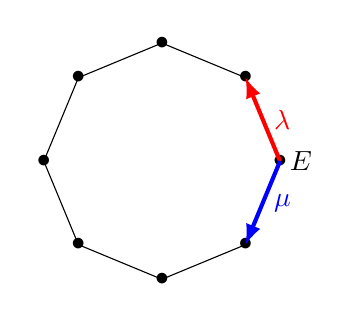
\begin{tikzpicture}[scale=0.3]
          \coordinate (A) at (0:5);
          \coordinate (B) at (45:5);
          \coordinate (C) at (90:5);
          \coordinate (D) at (135:5);
          \coordinate (E) at (180:5);
          \coordinate (F) at (225:5);
          \coordinate (G) at (270:5);
          \coordinate (H) at (315:5);
          \draw (A)--(B)--(C)--(D)--(E)--(F)--(G)--(H)--(A);	
          
          \draw (A) node[right]{$E$};
          \draw (A) node{$\bullet$};
          \draw (B) node{$\bullet$};
          \draw (C) node{$\bullet$};
          \draw (D) node{$\bullet$};
          \draw (E) node{$\bullet$};
          \draw (F) node{$\bullet$};
          \draw (G) node{$\bullet$};
          \draw (H) node{$\bullet$};
          
          \draw[line width=1.5pt,red,-latex] (A)--(B) node[midway,right]{$\color{red} \lambda$};
          \draw[line width=1.5pt,blue,-latex] (A)--(H) node[midway,right]{$\color{blue} \mu$};
        \end{tikzpicture}	
      \end{center}
    \end{figure}
  }

\end{frame}


%%%%%%%%%%%%%%%%%%%%%%%%%%%%%%%%%%%%%%%%%%%%%%%%%%%%%%%%%%%% 

\begin{frame}
  \orangebox{Fact}{
    Let $\phi$ be an $r$-isogeny with $\ell \nmid r$, then $\phi$ preserves the kernels of the $\ell$-isogenies of direction $\red \lambda, \blu \mu $.}

  To interpolate $\phi$ over $E[\ell^k]$, we want to compute two cyclic
  $\ell^k$-subgroups of direction $\red \lambda, \blu \mu $. 

  \begin{figure}[h]
    \begin{center}
      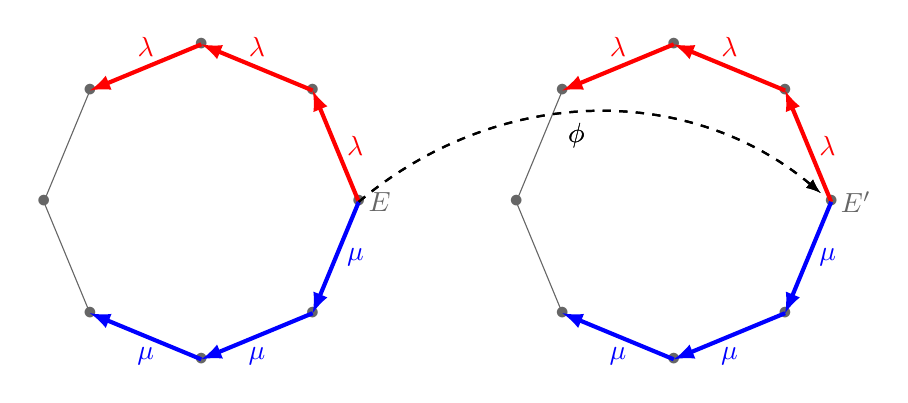
\begin{tikzpicture}[scale=0.4]
        \foreach \s/\e in {0/E,15cm/E'} {
          \begin{scope}[xshift=\s,black!60]
            \coordinate (A) at (0:5);
            \coordinate (B) at (45:5);
            \coordinate (C) at (90:5);
            \coordinate (D) at (135:5);
            \coordinate (E) at (180:5);
            \coordinate (F) at (225:5);
            \coordinate (G) at (270:5);
            \coordinate (H) at (315:5);

            \draw (A) node{$\bullet$};
            \draw (A) node[right]{$\e$};
            \draw (B) node{$\bullet$};
            \draw (C) node{$\bullet$};
            \draw (D) node{$\bullet$};
            \draw (E) node{$\bullet$};
            \draw (F) node{$\bullet$};
            \draw (G) node{$\bullet$};
            \draw (H) node{$\bullet$};

            \draw (A)--(B)--(C)--(D)--(E)--(F)--(G)--(H)--(A);		
            \begin{scope}[-latex]
              \draw[line width=1.5pt,red] (A)--(B) node[midway,right]{$\color{red} \lambda$};
              \draw[line width=1.5pt,blue] (A)--(H) node[midway,right]{$\color{blue} \mu$};
              \uncover<2->{
                \draw[line width=1.5pt,red] (B)--(C) node[midway,above]{$\color{red} \lambda$};
                \draw[line width=1.5pt,blue] (H)--(G) node[midway,below]{$\color{blue} \mu$};
              }
              \uncover<3->{
                \draw[line width=1.5pt,red] (C)--(D) node[midway,above]{$\color{red} \lambda$};
                \draw[line width=1.5pt,blue] (G)--(F) node[midway,below]{$\color{blue} \mu$};
              }
            \end{scope}
          \end{scope}

          \draw[dashed,thick,-latex,shorten >=5pt] (0:5) to[bend left=40] node[below left] {$\phi$} (0:20);
        }
      \end{tikzpicture}	
    \end{center}
  \end{figure}

  \begin{uncoverenv}<3->
    \begin{itemize}
    \item We call $\red{E[\ell^k]_\lambda}\oplus\blu{E[\ell^k]_\mu}$ a
      \emph{horizontal} decomposition;
    \item SEA literature calls this an \emph{isogeny cycle} [Couveignes, Morain '94].
    \end{itemize}
  \end{uncoverenv}

\end{frame}

%%%%%%%%%%%%%%%%%%%%%%%%%%%%%%%%%%%%%%%%%%%%%%%%%%%%%%%%%%%% 

\begin{frame}

  \orangebox{Towards an $\ell$-adic Couveignes' algorithm ($\pi$ splits modulo $\ell$)}{
    \begin{description}
    \item[Input:] $E, E'$ two $r$-isogenous curves on $\F_{q}$,
    \item[Output:] $\phi: E \rightarrow E'$ of degree $r$.
    \end{description}}

  \orangebox{}{\textbf{Fact:} $\phi$ maps 
    $\color{red}{E[\ell^k]_{{\lambda}}} \color{black}{\rightarrow} \color{red}{E'[\ell^k]_{{\lambda}}}$  
    and 
    $\color{blue}{E[\ell^k]_{{\mu}}} \color{black}{\rightarrow} \color{blue}{E'[\ell^k]_{{\mu}}}$.
  }

  \begin{enumerate}
  \item Select the least $k$ such that  $\ell^{2k}>4r$.
    \medskip
  \item Compute $\langle \red P , \blu Q \rangle = \color{red}{E[\ell^k]_{{\lambda}}} \color{black} \oplus \color{blue}{E[\ell^k]_{{\mu}}} $\\
    and $\langle \red P' , \blu Q' \rangle = \color{red}{E'[\ell^k]_{{\lambda}}} \color{black} \oplus \color{blue}{E'[\ell^k]_{{\mu}}} $
    % \item Deduce $\to$ $\langle{\color{red}P},{\color{blue}Q}\rangle=E[\ell^k]$ and $\langle{\color{red}P'},{\color{blue}Q'}\rangle=E'[\ell^k]$;
    \medskip
  \item For each \textbf{invertible diagonal} matrix
    $\left ( \begin{smallmatrix}a & 0\\ 0 & b
      \end{smallmatrix}\right )$ in $(\mathbb{Z}/\ell^k \mathbb{Z})^{2 \times 2}$:
    \hfill\only<2>{$O(r)$}
    \begin{enumerate}

    \item Compute the interpolation polynomial
      $L$ sending\\
      $\color{red}P\mapsto aP'$ and $\color{blue}Q\mapsto bQ'$;
      \hfill\only<2>{$\tilde{O}(r \ell^{O(1)})$}
    \item Use a  rational reconstruction  algorithm 
      to compute a rational
      fraction $F$ of degrees~$(r, r-1)$;
      \hfill\only<2>{$\tilde{O}(r)$}
    \item If $F$ defines an isogeny of degree $r$, return it and
      stop.
    \end{enumerate}
  \end{enumerate}
\end{frame}

%%%%%%%%%%%%%%%%%%%%%%%%%%%%%%%%%%%%%%%%%%%%%%%%%%%%%%%%%%%% 

\begin{frame}
  \begin{center}
    \Huge 
    \uncover<1>{I'm done. Thanks.}

    \uncover<2>{Questions?}

    \uncover<3>{No?}

    \uncover<4->{Ok, wait, I'm not done yet!}
  \end{center}
\end{frame}

%%%%%%%%%%%%%%%%%%%%%%%%%%%%%%%%%%%%%%%%%%%%%%%%%%%%%%%%%%%% 
%%%%%%%%%%%%%%%%%%%%%%%%%%%%%%%%%%%%%%%%%%%%%%%%%%%%%%%%%%%% 
\section{An $\ell$-adic Couveignes algorithm}

\begin{frame}
  \frametitle{Towards the general case}

  Denote by $\mathcal{O}$ (resp. $\mathcal{O}'$) the endomorphism ring of $E$ (resp. $E'$)
  \vspace{-4mm}
  \begin{columns}
    \begin{column}{6cm}
      \only<1-1>{
        \begin{figure}
          \begin{center}

            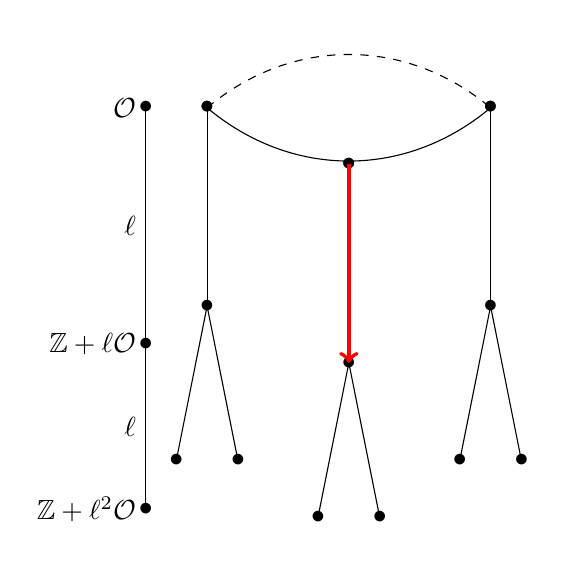
\begin{tikzpicture}[scale=0.60]
              \coordinate (A) at (0,1.5);
              \coordinate (AB) at (1,1.5);
              % \coordinate (AZ) at (-1.5,1.5);	
              \coordinate (B) at (0,5);
              \coordinate (BB) at (1,5);
              % \coordinate (BZ) at (-1.5,5.2);
              % \coordinate (BZ2) at (-1.5,4.8);
              \coordinate (C) at (0,10);
              \coordinate (CB) at (1,10);
              % \coordinate (CZ) at (-1.5,10);
              \draw (A) node[left]{$\mathbb{Z} + \ell^2 \mathcal{O}$} node{$\bullet$};
              \draw (B) node[left]{$\mathbb{Z} + \ell \mathcal{O}$} node{$\bullet$};
              \draw (C) node[left]{$\mathcal{O}$} node{$\bullet$};
              \draw (A)--(B)node[midway,left] {$\ell$};
              \draw (B)--(C) node[midway,left] {$\ell$};
              % \draw (CZ)--(BZ)[dashed]  node[midway,left] {$\ell$};
              % \draw (BZ2)--(AZ)[dashed]  node[midway,left] {$\ell$};
              \begin{scope}[yshift=10cm]
                \begin{scope}[xshift=4.3cm]
                  \node (A) at (-3,0) {$\bullet$};
                  \node (B) at (3,0) {$\bullet$};
                  \node (C) at (270:1.2) {$\bullet$};
                  \node (D) at (90:1.5) {};
                  % \draw[-] (A.center) to[bend right=25] (C.center);
                  \draw[-,dashed] (A.center) to[bend left=40] (B.center);
                  % \draw[-] (B.center) to[bend left=25] (C.center);
                  % \draw[-,dashed] (B.center) to[bend right] (D.center);
                  \draw[-] (A.center) to[bend right=40] (B.center);
                  \begin{scope}[xshift=-3cm]
                    \coordinate (A) at (0,0);
                    \coordinate (C) at (270:4.2);
                    \coordinate (CA) at (265:7.5);
                    \coordinate (CB) at (275:7.5);
                    \draw (C)--(CA);
                    \draw (C)--(CB);
                    \draw (CA) node{$\bullet$};
                    \draw (CB) node{$\bullet$};
                    \draw (A) node{$\bullet$};
                    \draw (C) node{$\bullet$};
                    \draw (A)--(C);
                  \end{scope}
                  \begin{scope}[xshift=3cm]
                    \coordinate (A) at (0,0);
                    \coordinate (C) at (270:4.2);
                    \coordinate (CA) at (265:7.5);
                    \coordinate (CB) at (275:7.5);
                    \draw (C)--(CA);
                    \draw (C)--(CB);
                    \draw (CA) node{$\bullet$};
                    \draw (CB) node{$\bullet$};
                    \draw (A) node{$\bullet$};
                    \draw (C) node{$\bullet$};
                    \draw (A)--(C);
                  \end{scope}
                  \begin{scope}[yshift=-1.2cm]
                    \coordinate (A) at (0,0);
                    \coordinate (C) at (270:4.2);
                    \coordinate (CA) at (265:7.5);
                    \coordinate (CB) at (275:7.5);
                    \draw (C)--(CA);
                    \draw (C)--(CB);
                    \draw (CA) node{$\bullet$};
                    \draw (CB) node{$\bullet$};
                    \draw (A) node{$\bullet$};
                    \draw (C) node{$\bullet$};
                    \draw[line width=1.5pt,red,->] (A)--(C);
                  \end{scope}
                \end{scope}
              \end{scope}
            \end{tikzpicture}
          \end{center}		
        \end{figure}}

      \only<2-2>{
        \begin{figure}
          \begin{center}

            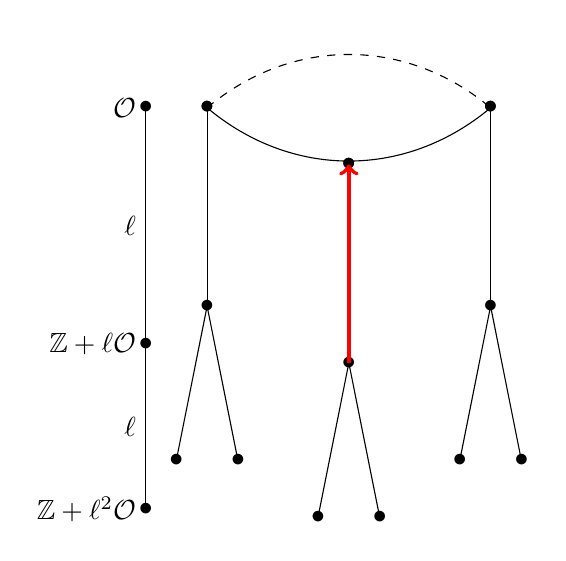
\begin{tikzpicture}[scale=0.60]
              \coordinate (A) at (0,1.5);
              \coordinate (AB) at (1,1.5);
              % \coordinate (AZ) at (-1.5,1.5);	
              \coordinate (B) at (0,5);
              \coordinate (BB) at (1,5);
              % \coordinate (BZ) at (-1.5,5.2);
              % \coordinate (BZ2) at (-1.5,4.8);
              \coordinate (C) at (0,10);
              \coordinate (CB) at (1,10);
              % \coordinate (CZ) at (-1.5,10);
              \draw (A) node[left]{$\mathbb{Z} + \ell^2 \mathcal{O}$} node{$\bullet$};
              \draw (B) node[left]{$\mathbb{Z} + \ell \mathcal{O}$} node{$\bullet$};
              \draw (C) node[left]{$\mathcal{O}$} node{$\bullet$};
              \draw (A)--(B)node[midway,left] {$\ell$};
              \draw (B)--(C) node[midway,left] {$\ell$};
              % \draw (CZ)--(BZ)[dashed]  node[midway,left] {$\ell$};
              % \draw (BZ2)--(AZ)[dashed]  node[midway,left] {$\ell$};
              \begin{scope}[yshift=10cm]
                \begin{scope}[xshift=4.3cm]
                  \node (A) at (-3,0) {$\bullet$};
                  \node (B) at (3,0) {$\bullet$};
                  \node (C) at (270:1.2) {$\bullet$};
                  \node (D) at (90:1.5) {};
                  % \draw[-] (A.center) to[bend right=25] (C.center);
                  \draw[-,dashed] (A.center) to[bend left=40] (B.center);
                  % \draw[-] (B.center) to[bend left=25] (C.center);
                  % \draw[-,dashed] (B.center) to[bend right] (D.center);
                  \draw[-] (A.center) to[bend right=40] (B.center);
                  \begin{scope}[xshift=-3cm]
                    \coordinate (A) at (0,0);
                    \coordinate (C) at (270:4.2);
                    \coordinate (CA) at (265:7.5);
                    \coordinate (CB) at (275:7.5);
                    \draw (C)--(CA);
                    \draw (C)--(CB);
                    \draw (CA) node{$\bullet$};
                    \draw (CB) node{$\bullet$};
                    \draw (A) node{$\bullet$};
                    \draw (C) node{$\bullet$};
                    \draw (A)--(C);
                  \end{scope}
                  \begin{scope}[xshift=3cm]
                    \coordinate (A) at (0,0);
                    \coordinate (C) at (270:4.2);
                    \coordinate (CA) at (265:7.5);
                    \coordinate (CB) at (275:7.5);
                    \draw (C)--(CA);
                    \draw (C)--(CB);
                    \draw (CA) node{$\bullet$};
                    \draw (CB) node{$\bullet$};
                    \draw (A) node{$\bullet$};
                    \draw (C) node{$\bullet$};
                    \draw (A)--(C);
                  \end{scope}
                  \begin{scope}[yshift=-1.2cm]
                    \coordinate (A) at (0,0);
                    \coordinate (C) at (270:4.2);
                    \coordinate (CA) at (265:7.5);
                    \coordinate (CB) at (275:7.5);
                    \draw (C)--(CA);
                    \draw (C)--(CB);
                    \draw (CA) node{$\bullet$};
                    \draw (CB) node{$\bullet$};
                    \draw (A) node{$\bullet$};
                    \draw (C) node{$\bullet$};
                    \draw[line width=1.5pt,red,<-] (A)--(C);
                  \end{scope}
                \end{scope}
              \end{scope}
            \end{tikzpicture}
          \end{center}		
        \end{figure}}

      \only<3-3>{
        \begin{figure}
          \begin{center}

            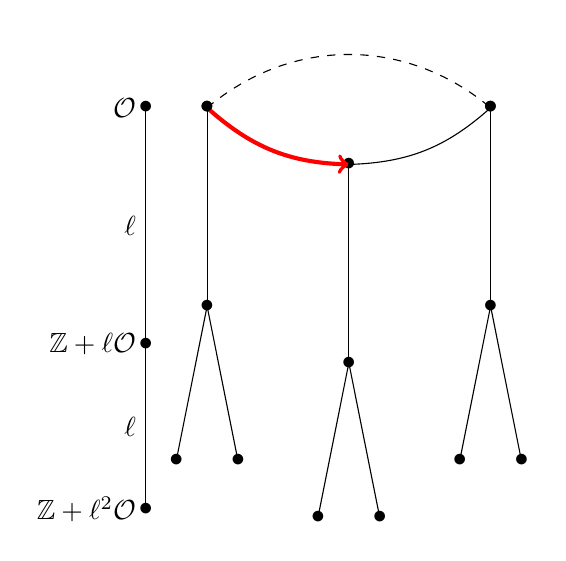
\begin{tikzpicture}[scale=0.60]
              \coordinate (A) at (0,1.5);
              \coordinate (AB) at (1,1.5);
              % \coordinate (AZ) at (-1.5,1.5);	
              \coordinate (B) at (0,5);
              \coordinate (BB) at (1,5);
              % \coordinate (BZ) at (-1.5,5.2);
              % \coordinate (BZ2) at (-1.5,4.8);
              \coordinate (C) at (0,10);
              \coordinate (CB) at (1,10);
              % \coordinate (CZ) at (-1.5,10);
              \draw (A) node[left]{$\mathbb{Z} + \ell^2 \mathcal{O}$} node{$\bullet$};
              \draw (B) node[left]{$\mathbb{Z} + \ell \mathcal{O}$} node{$\bullet$};
              \draw (C) node[left]{$\mathcal{O}$} node{$\bullet$};
              \draw (A)--(B)node[midway,left] {$\ell$};
              \draw (B)--(C) node[midway,left] {$\ell$};
              % \draw (CZ)--(BZ)[dashed]  node[midway,left] {$\ell$};
              % \draw (BZ2)--(AZ)[dashed]  node[midway,left] {$\ell$};
              \begin{scope}[yshift=10cm]
                \begin{scope}[xshift=4.3cm]
                  \node (A) at (-3,0) {$\bullet$};
                  \node (B) at (3,0) {$\bullet$};
                  \node (C) at (270:1.2) {$\bullet$};
                  \node (D) at (90:1.5) {};
                  % \draw[-] (A.center) to[bend right=25] (C.center);
                  \draw[-,dashed] (A.center) to[bend left=40] (B.center);
                  % \draw[-] (B.center) to[bend left=25] (C.center);
                  % \draw[-,dashed] (B.center) to[bend right] (D.center);
                  \draw[-] (C.center) to[bend right=20] (B.center);
                  \draw[line width=1.5pt,red,->] (A.center) to[bend right=20] (C.center);
                  \begin{scope}[xshift=-3cm]
                    \coordinate (A) at (0,0);
                    \coordinate (C) at (270:4.2);
                    \coordinate (CA) at (265:7.5);
                    \coordinate (CB) at (275:7.5);
                    \draw (C)--(CA);
                    \draw (C)--(CB);
                    \draw (CA) node{$\bullet$};
                    \draw (CB) node{$\bullet$};
                    \draw (A) node{$\bullet$};
                    \draw (C) node{$\bullet$};
                    \draw (A)--(C);
                  \end{scope}
                  \begin{scope}[xshift=3cm]
                    \coordinate (A) at (0,0);
                    \coordinate (C) at (270:4.2);
                    \coordinate (CA) at (265:7.5);
                    \coordinate (CB) at (275:7.5);
                    \draw (C)--(CA);
                    \draw (C)--(CB);
                    \draw (CA) node{$\bullet$};
                    \draw (CB) node{$\bullet$};
                    \draw (A) node{$\bullet$};
                    \draw (C) node{$\bullet$};
                    \draw (A)--(C);
                  \end{scope}
                  \begin{scope}[yshift=-1.2cm]
                    \coordinate (A) at (0,0);
                    \coordinate (C) at (270:4.2);
                    \coordinate (CA) at (265:7.5);
                    \coordinate (CB) at (275:7.5);
                    \draw (C)--(CA);
                    \draw (C)--(CB);
                    \draw (CA) node{$\bullet$};
                    \draw (CB) node{$\bullet$};
                    % \draw (A) node{$\bullet$};
                    \draw (C) node{$\bullet$};
                    \draw (A)--(C);
                  \end{scope}
                \end{scope}
              \end{scope}
            \end{tikzpicture}
          \end{center}		
        \end{figure}}


    \end{column}
    \begin{column}{4cm}

      \begin{lem}[Kohel 1996]
        $E$ and $E'$ two elliptic curves defined over $\F_q$, $\psi :E \rightarrow E'$ an $\ell$-isogeny. Then we say that $\psi$ is
        \begin{enumerate}
        \item  \textbf<1>{descending} if $\ell=[\mathcal{O} : \mathcal{O}']$
        \item \textbf<2>{ascending} if $\ell=[\mathcal{O}':\mathcal{O}]$,
        \item \textbf<3>{horizontal} if $\mathcal{O}=\mathcal{O}'$.
        \end{enumerate}
      \end{lem}
      % \begin{defi}
      %   The index $f=[\mathcal{O}_K : \mathcal{O}]$ is called the conductor of $\mathcal{O}$.
      % \end{defi}
    \end{column}

  \end{columns}
\end{frame}


%%%%%%%%%%%%%%%%%%%%%%%%%%%%%%%%%%%%%%%%%%%%%%%%%%%%%%%%%%%% 

\begin{frame}
  \frametitle{A guide to volcano types}
  \begin{figure}[h]
    \begin{center}
      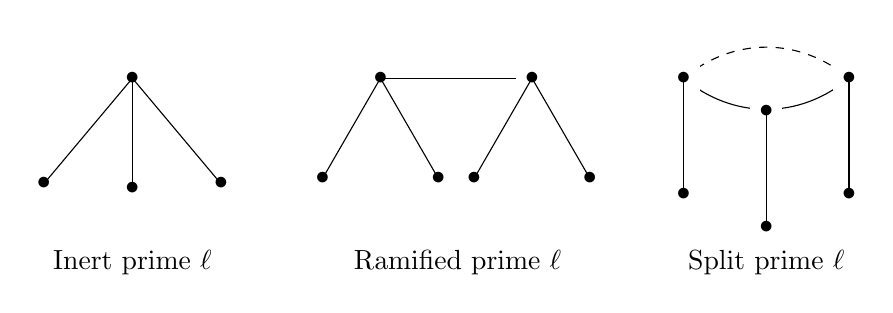
\begin{tikzpicture}[scale=0.35]
        \coordinate (A) at (0,0);
        \coordinate (B) at (230:5);
        \coordinate (C) at (270:4);
        \coordinate (D) at (310:5);
        \draw (A) node{$\bullet$};
        \draw (B) node[fill=white]{$\bullet$};
        \draw (C) node[fill=white]{$\bullet$};
        \draw (D) node[fill=white]{$\bullet$};
        \node at (0,-6.7) {Inert prime $\ell$};
        \draw (A)--(B);
        \draw (A)--(C);
        \draw (A)--(D);		
        \begin{scope}[xshift=9cm]
          \coordinate (A) at (0,0);
          \coordinate (B) at (5.5,0);
          \coordinate (C) at (240:4.2);
          \coordinate (D) at (300:4.2);
          \draw (A) node[fill=white]{$\bullet$};
          \draw (B) node[fill=white]{$\bullet$};
          \draw (C) node[fill=white]{$\bullet$};
          \draw (D) node[fill=white]{$\bullet$};
          \node at (2.8,-6.7) {Ramified prime $\ell$};
          \draw (A)--(B);
          \draw (A)--(C);
          \draw (A)--(D);
        \end{scope}
        
        \begin{scope}[xshift=14.5cm]
          \coordinate (A) at (0,0);
          \coordinate (C) at (240:4.2);
          \coordinate (D) at (300:4.2);
          \draw (A) node[fill=white]{$\bullet$};
          \draw (C) node[fill=white]{$\bullet$};
          \draw (D) node[fill=white]{$\bullet$};
          \draw (A)--(C);
          \draw (A)--(D);
        \end{scope}
        
        \begin{scope}[xshift=23cm]
          \node (A) at (-3,0) {$\bullet$};
          \node (B) at (3,0) {$\bullet$};
          \node (C) at (270:1.2) {$\bullet$};
          \node (D) at (90:1.5) {};
          \node at (0,-6.7) {Split prime $\ell$};
          % \draw[-] (A.center) to[bend right=25] (C.center);
          \draw[-,dashed] (A.center) to[bend left=40] (B.center);
          % \draw[-] (B.center) to[bend left=25] (C.center);
          % \draw[-,dashed] (B.center) to[bend right] (D.center);
          \draw[-] (A.center) to[bend right=40] (B.center);
          \begin{scope}[xshift=-3cm]
            \coordinate (A) at (0,0);
            \coordinate (C) at (270:4.2);
            \draw (A) node[fill=white]{$\bullet$};
            \draw (C) node[fill=white]{$\bullet$};
            \draw (A)--(C);
          \end{scope}
          \begin{scope}[xshift=3cm]
            \coordinate (A) at (0,0);
            \coordinate (C) at (270:4.2);
            \draw (A) node[fill=white]{$\bullet$};
            \draw (C) node[fill=white]{$\bullet$};
            \draw (A)--(C);
          \end{scope}
          \begin{scope}[yshift=-1.2cm]
            \coordinate (A) at (0,0);
            \coordinate (C) at (270:4.2);
            \draw (A) node[fill=white]{$\bullet$};
            \draw (C) node[fill=white]{$\bullet$};
            \draw (A)--(C);
          \end{scope}
        \end{scope}
      \end{tikzpicture}
      % \end{center}
      \caption{The three shapes of volcanoes of $2$-isogenies }
      
    \end{center} 
  \end{figure}
  In the rest of this talk we consider only volcanoes with cyclic crater (Elkies case).
\end{frame}

%%%%%%%%%%%%%%%%%%%%%%%%%%%%%%%%%%%%%%%%%%%%%%%%%%%%%%%%%%%% 
\begin{frame}{The Elkies case}

  \orangebox{Elkies prime}{We say that $\ell$ is an \emph{Elkies prime} if the characteristic polynomial of $\pi$ factors over $\mathbb{Z}_{\ell}$ as
    \[
      \pi^2 - t_{\pi}\pi + q = (\pi - \red \lambda) (\pi - \blu \mu), \quad \textsf{with } \red \lambda \neq \blu \mu,
    \]
    where $h=v_{\ell}(\red \lambda - \blu \mu)$ can be $\geqslant 1$.
  }

  \emph{Note:} $h=v_\ell(\red \lambda - \blu \mu)$ is the height of
  the $\ell$-volcano.

  \bigskip

  \emph{Problem:} as long as $k\le h$, the two eigenvalues are
  \alert{undistinguishable}:
  \[
    \pi(P)=\red \lambda P = \blu \mu P
    \quad\text{for any $P\in E[\ell^h].$}
  \]
  
  From now on, we assume\footnote{This has no impact on the complexity
    as the isogeny degree grows, indeed $k\approx\log(r)$.} that
  $k \geqslant h+1$.
\end{frame}

%

\begin{frame}

  \begin{prop}[LDF, Hugounenq, Plût, Schost]\label{prop:matrice-Frobenius}
    In the Elkies case the action of the Frobenius endomorphism $\pi$ on $E[\ell^{h+1}]$~is conjugate, over~$\mathbb{Z}_{\ell}$,
    to a unique matrix \[\left ( \begin{matrix}{\color{red}\lambda} & a\\ 0 &
          {\color{blue}\mu} \end{matrix}\right ), \]  with $a \in \{ 1,\ell, \dots,
    \ell^{h-1}, 0  \}$, and $a = 0$ iff~$E$ lies on the crater.
  \end{prop}

  \begin{figure}
    \begin{center}

      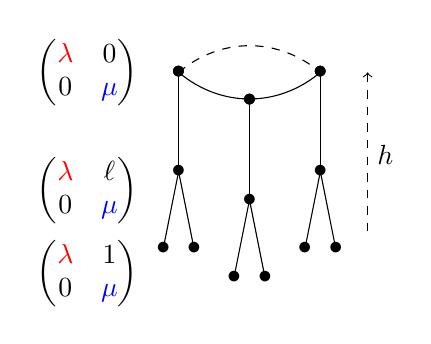
\begin{tikzpicture}[scale=0.30]
        \coordinate (A) at (0,1.5);
        \coordinate (AB) at (1,1.5);
        \coordinate (AZ) at (-1.5,1.5);	
        \coordinate (B) at (0,5);
        \coordinate (BB) at (1,5);
        \coordinate (BZ) at (-1.5,5.2);
        \coordinate (BZ2) at (-1.5,4.8);
        \coordinate (C) at (0,10);
        \coordinate (CB) at (1,10);
        \coordinate (CZ) at (-1.5,10);
        \draw (A) node[left]{$\left( \begin{matrix}
              \color{red}{\lambda} & 1 \\
              0 & \color{blue}{\mu}
            \end{matrix} \right) \color{black} $}; %node{$\bullet$};
        \draw (B) node[left]{$ \left( \begin{matrix}
              \color{red}{\lambda} & \ell \\
              0 & \color{blue}{\mu}
            \end{matrix} \right) \color{black} $}; %node{$\bullet$};
        \draw (C) node[left]{$ \left( \begin{matrix}
              \color{red}{\lambda} & 0 \\
              0 & \color{blue}{\mu}
            \end{matrix} \right) \color{black} $}; %node{$\bullet$};
        % \draw (A)--(B);
        % \draw (B)--(C);
        % \draw (CZ)--(BZ)[dashed]  node[midway,left] {$\ell$};
        % \draw (BZ2)--(AZ)[dashed]  node[midway,left] {$\ell$};
        \begin{scope}[yshift=10cm]
          \begin{scope}[xshift=4.3cm]
            \node (A) at (-3,0) {$  \bullet $};
            \node (B) at (3,0) {$   \bullet$};
            \node (C) at (270:1.2) {$ \bullet \color{black}$};
            \node (D) at (90:1.5) {};
            % \draw[-] (A.center) to[bend right=25] (C.center);
            \draw[-,dashed] (A.center) to[bend left=40] (B.center);
            % \draw[-] (B.center) to[bend left=25] (C.center);
            % \draw[-,dashed] (B.center) to[bend right] (D.center);
            \draw[-] (A.center) to[bend right=40] (B.center);
            \draw (A) node{$  \bullet $};
            \draw (B) node{$  \bullet $};
            \draw (C) node{$  \bullet $};
            % \draw[line width=2.5pt,red,->] (A.center) to[bend right=20] (C.center);
            \begin{scope}[xshift=-3cm]
              \coordinate (A) at (0,0);
              \coordinate (C) at (270:4.2);
              \coordinate (CA) at (265:7.5);
              \coordinate (CB) at (275:7.5);
              \draw (C)--(CA);
              \draw (C)--(CB);
              \draw (A)--(C);
              \draw (CA) node{$ \bullet$};
              \draw (CB) node{$\bullet$};
              \draw (A) node{$  \bullet \color{black}$};
              \draw (C) node{$  \bullet \color{black}$};
            \end{scope}
            \begin{scope}[xshift=3cm]
              \coordinate (A) at (0,0);
              \coordinate (C) at (270:4.2);
              \coordinate (CA) at (265:7.5);
              \coordinate (CB) at (275:7.5);
              \draw (C)--(CA);
              \draw (C)--(CB);
              \draw (A)--(C);
              \draw (CA) node{$ \bullet$};
              \draw (CB) node{$\bullet$};
              \draw (A) node{$ \bullet$};
              \draw (C) node{$ \bullet$};
            \end{scope}
            \begin{scope}[yshift=-1.2cm]
              \coordinate (A) at (0,0);
              \coordinate (C) at (270:4.2);
              \coordinate (CA) at (265:7.5);
              \coordinate (CB) at (275:7.5);
              \draw (C)--(CA);
              \draw (C)--(CB);
              \draw (A)--(C);
              \draw (CA) node{$ \bullet$};
              \draw (CB) node{$ \bullet$};
              % \draw (A) node{$\bullet$};
              \draw (C) node{$ \bullet$};
              \draw (A) node{$ \bullet$};
              
              
              % (C) node[left]{$\mathcal{O}$} node{$\bullet$};			
              
            \end{scope}
            \coordinate (F) at (5,0);
            \coordinate (G) at (5,-7);
            \draw[dashed,<-] (F)--(G) node[midway,right]{$h$};
          \end{scope}
        \end{scope}

      \end{tikzpicture}
    \end{center}
  \end{figure}
\end{frame}

%%%%%%%%%%%%%%%%%%%%%%%%%%%%%%%%%%%%%%%%%%%%%%%%%%%%%%%%%%%% 


\begin{frame}
  Suppose that $E$ lies on the crater (we can reduce to this case easily).
  
  \begin{columns}
    \begin{column}{5cm}
      \orangebox{Volcano with height $h=0$}{
        \begin{figure}[h]
          \begin{center}
            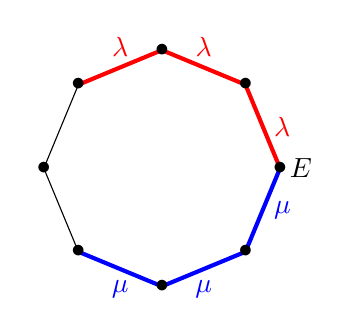
\begin{tikzpicture}[scale=0.3]
              \coordinate (A) at (0:5);
              \coordinate (B) at (45:5);
              \coordinate (C) at (90:5);
              \coordinate (D) at (135:5);
              \coordinate (E) at (180:5);
              \coordinate (F) at (225:5);
              \coordinate (G) at (270:5);
              \coordinate (H) at (315:5);
              \draw (A)--(B)--(C)--(D)--(E)--(F)--(G)--(H)--(A);		
              \draw[line width=1.5pt,red] (A)--(B) node[midway,right]{$\color{red} \lambda$};
              \draw[line width=1.5pt,blue] (A)--(H) node[midway,right]{$\color{blue} \mu$};
              \draw[line width=1.5pt,red] (B)--(C) node[midway,above]{$\color{red} \lambda$};
              \draw[line width=1.5pt,blue] (H)--(G) node[midway,below]{$\color{blue} \mu$};
              \draw[line width=1.5pt,red] (C)--(D) node[midway,above]{$\color{red} \lambda$};
              \draw[line width=1.5pt,blue] (G)--(F) node[midway,below]{$\color{blue} \mu$};
              
              \draw (A) node[right]{$E$};
              \draw (A) node{$\bullet$};
              \draw (B) node{$\bullet$};
              \draw (C) node{$\bullet$};
              \draw (D) node{$\bullet$};
              \draw (E) node{$\bullet$};
              \draw (F) node{$\bullet$};
              \draw (G) node{$\bullet$};
              \draw (H) node{$\bullet$};
            \end{tikzpicture}	
          \end{center}
        \end{figure}
      }
      \begin{itemize}
      \item $\ker(\pi- \blu \mu\; | \; E[\ell^k])$ is cyclic
        of size $\ell^k$;
      \item Interpolation maps a cyclic group to a cyclic group;
      \item $O(\ell^k)$ choices. Happiness!
      \end{itemize}
    \end{column}
    \begin{column}{5.5cm}
      \orangebox{Volcano with height $h=2$}{\begin{center}
          \tikzstyle{lambda1}=[lambda,draw=blue!60!green]
          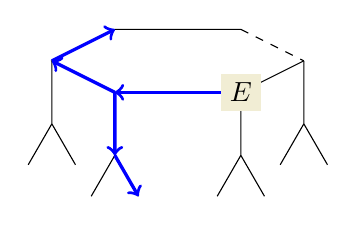
\begin{tikzpicture}[scale=0.40]
            % \coordinate (A) at (0,-1.2);
            % \coordinate (B) at (-3,0);
            % \coordinate (C) at (-1.2,.7);
            % \coordinate (D) at (1.2,.7);
            % \coordinate (E) at (3,0);
            \coordinate (A) at (2,-1);
            \coordinate (B) at (-2,-1);
            \coordinate (C) at (-4,0);
            \coordinate (D) at (-2,1);
            \coordinate (E) at (2,1);
            \coordinate (F) at (4,0);
            \draw (F)--(A)--(B)--(C)--(D)--(E); \draw[dashed] (E)--(F);

            \coordinate[position=-90:.8 from A] (AA);
            \coordinate[position=-60:.6 from AA] (AA0);
            \coordinate[position=-120:.6 from AA] (AA1);
            \draw (A)--(AA)--(AA0); \draw (AA)--(AA1);
            \coordinate[position=-90:.8 from B] (BB);
            \coordinate[position=-60:.6 from BB] (BB0);
            \coordinate[position=-120:.6 from BB] (BB1);
            \draw (B)--(BB)--(BB0); \draw (BB)--(BB1);
            \coordinate[position=-90:.8 from C] (CC);
            \coordinate[position=-60:.6 from CC] (CC0);
            \coordinate[position=-120:.6 from CC] (CC1);
            \draw (C)--(CC)--(CC0); \draw (CC)--(CC1);
            \coordinate[position=-90:.8 from F] (FF);
            \coordinate[position=-60:.6 from FF] (FF0);
            \coordinate[position=-120:.6 from FF] (FF1);
            \draw (F)--(FF)--(FF0); \draw (FF)--(FF1);
            \draw[lambda] (A)--(B);
            \draw<1>[lambda] (B)--(C);
            \draw<1>[lambda] (C)--(D);
            \draw<2->[lambda] (B)--(BB);
            \draw<2->[lambda] (BB)--(BB0);
            \node[fill=pacificcream] at (A) {$E$};
          \end{tikzpicture}
        \end{center}
      }
      \textbf{Problem:} 
      \begin{itemize}
      \item
        $\ker(\pi- \blu \mu \;| \; E[\ell^k]) \simeq (\mathbb
        Z/\ell^k) \!\times\! (\mathbb Z/\ell^h)$;
      \item It contains $\ell^h$ cyclic subgroups of order $\ell^k$;
      \item Each cyclic subgroup is associated to an isogeny that
        \textbf{starts} horizontal;
      \item $O(\ell^{k+h})$ choices. Sadness.
      \end{itemize}
    \end{column}
  \end{columns}

\end{frame}


%%%%%%%%%%%%%%%%%%%%%%%%%%%%%%%%%%%%%%%%%%%%%%%%%%%%%%%%%%%% 

\begin{frame}
  \frametitle{Walking on the crater}
  
  \begin{columns}
    \begin{column}{0.5\textwidth}
      \emph{Trivial fix:} compute a basis of $E[\ell^{k+h}]$, only to
      obtain only a horizontal decomposition of $E[\ell^k]$.
      
      \bigskip

      \emph{\textbf{Much better:}}
      \begin{enumerate}
      \item Start with \textbf{any} walk of length $k\ge h+1$;
      \item First step is horizontal, use it to move to the next curve;
      \item Compute again a walk of length $k$ (actually only requires computing
        one step);
      \item etc.
      \end{enumerate}
    \end{column}
    \begin{column}{0.4\textwidth}
      \begin{tikzpicture}[scale=0.50]
        \begin{scope}[yshift=10cm]
          \begin{scope}[xshift=4.3cm]
            \node (A) at (-3,0) {$\bullet$};
            \node (B) at (3,0) {$\bullet$};
            \node (C) at (270:1.2) {$\bullet$};
            \node (D) at (125:1.2) {$E_2$};
            % \draw[-] (A.center) to[bend right=25] (C.center);
            \draw[-] (D.center) to[bend right=20] (A.center);
            \only<1-2>{		
              \draw[-] (D.center) to[bend left=18] (B.center);
            }
            \only<3->{
              \draw[line width=1.5pt,blue,->] (D.center) to[bend left=20] (B.center);
              
              \node (F) at (1.25,1.30) {$\color{blue} \mu$};
              % \node (F2) at (1.25,0.50) {$\color{blue} \psi_2$};		
            }
            \only<5->{
              \draw[line width=1.5pt,blue,->] (D.center) to[bend right=20] (A.center);		
            }
            \only<5->{		
              \node (F2) at (-2.25,1) {$\color{blue} \mu$};
            }
            % \only<4->{
            % \draw[line width=1.5pt,red,->] (D.center) to[bend left=20] (B.center);
            % \draw[-] (D.center) to[bend right=20] (A.center);
            % \node (F) at (1.25,1.30) {$\color{red} \lambda$};		
            % }
            %   \draw[-] (B.center) to[bend left=25] (C.center);
            %   \draw[-,dashed] (B.center) to[bend right] (D.center);
            \only<1->{
              \draw[line width=1.5pt,blue,->] (C.center) to[bend right=20] (B.center); 
              \node (F) at (1.5,-0.5) {$\color{blue} \mu$};	
              % \node (F2) at (1.5,-1.5) {$\color{blue} \psi$};	
            }
            % \only<2->{
            % \draw[line width=1.5pt,red,<-] (C.center) to[bend right=20] (B.center); 
            % \node (F) at (1.5,-0.5) {$\color{red} \lambda$};		
            % }
            
            \begin{scope}[xshift=-3cm]
              \coordinate (A) at (0,0);
              \coordinate (C) at (270:4.2);
              \coordinate (CA) at (265:7.5);
              \coordinate (CB) at (275:7.5);
              \draw (C)--(CA);
              \only<1>{
                \draw (C)--(CB);}
              \only<2->{
                \draw (C)--(CB);}
              \only<1-3>{			
                \draw (A)--(C);}
              \only<4->{
                \draw (A)--(C);}
              \only<5>{
                \draw [line width=1.5pt,blue] (C)--(A);
                \draw [line width=1.5pt,blue] (C)--(CA);
              }
              % just to have a 6th slide
              \only<6>{
                \draw (C)--(A);
                \draw (C)--(CA);
              }
              % \draw (A) node[fill=white]{$30$};
              % \draw (C) node[fill=white]{$98$};
              % \draw (CA) node[fill=white]{$22$};
              % \draw (CB) node[fill=white]{$74$};
              \draw (A) node[fill=white]{$E_3$};
              \draw (C) node[fill=white]{$\bullet$};
              \draw (CA) node[fill=white]{$\bullet$};
              \draw (CB) node[fill=white]{$\bullet$};
            \end{scope}
            \begin{scope}[xshift=3cm]
              \coordinate (A) at (0,0);
              \coordinate (C) at (270:4.2);
              \coordinate (CA) at (265:7.5);
              \coordinate (CB) at (275:7.5);
              \draw (C)--(CA);
              \draw (C)--(CB);
              \draw (A)--(C);
              \only<1>{
                \draw [line width=1.5pt,blue] (C)--(CB);
                \draw [line width=1.5pt,blue] (A)--(C);
              }
              % \draw (A) node[fill=white]{$65$};
              % \draw (C) node[fill=white]{$60$};
              % \draw (CA) node[fill=white]{$39$};
              % \draw (CB) node[fill=white]{$62$};
              \draw (A) node[fill=white]{$E_1$};
              \only<2-3>{\draw (A) node[fill=yellow!50!white,shape=circle]{$E_1$};}
              \draw (C) node[fill=white]{$\bullet$};
              \draw (CA) node[fill=white]{$\bullet$};
              \draw (CB) node[fill=white]{$\bullet$};
            \end{scope}
            \begin{scope}[yshift=-1.2cm]
              \coordinate (A) at (0,0);
              \coordinate (C) at (270:4.2);
              \coordinate (CA) at (265:7.5);
              \coordinate (CB) at (275:7.5);
              \draw (C)--(CA);
              \draw (C)--(CB);
              \draw (A)--(C);
              \draw (A) node[fill=white]{$E$};
              \only<1>{\draw (A) node[fill=yellow!50!white,shape=circle]{$E$};}
              \draw (C) node[fill=white]{$\bullet$};
              \draw (CA) node[fill=white]{$\bullet$};
              \draw (CB) node[fill=white]{$\bullet$};
              % \draw (CA) node[fill=white]{$45$};
              % \draw (CB) node[fill=white]{$68$};
            \end{scope}
            \begin{scope}[shift={(D)}]
              \coordinate (A) at (0,0);
              \coordinate (C) at (270:4.2);
              \coordinate (CA) at (265:7.5);
              \coordinate (CB) at (275:7.5);
              \draw [dashed] (C)--(CA);
              \draw [dashed] (C)--(CB);
              \draw [dashed] (A)--(C);
              \draw (C) node[color=black!90]{$\bullet$};
              \draw (CA) node[color=black!90]{$\bullet$};
              \draw (CB) node[color=black!90]{$\bullet$};
              \only<3>{
                \draw [line width=1.5pt,blue] (C)--(A);
                \draw [line width=1.5pt,blue] (C)--(CA);
              }
              \only<1-3,5->{\draw (A) node[fill=white]{$E_2$};}			
              \only<4>{\draw (A) node[fill=yellow!50!white,shape=circle]{$E_2$};}
            \end{scope}
            \coordinate (A) at (-3,0);
            \coordinate (C) at (270:1.2);
            \only<1->{
              \draw (A.center) to[bend right=20] (C.center);
            }
            \draw (A) node[fill=white]{$E_3$};
            \only<1>{
              \draw (C) node[fill=yellow!50!white,shape=circle]{$E$};
            }	
            \only<2->{
              \draw (C) node[fill=white]{$E$};
            }
          \end{scope}
        \end{scope}

      \end{tikzpicture}
    \end{column}
  \end{columns}
\end{frame}

%%%%%%%%%%%%%%%%%%%%%%%%%%%%%%%%%%%%%%%%%%%%%%%%%%%%%%%%%%%% 

\begin{frame}
  \frametitle{Details I glossed over}

  \orangebox{Computing in towers of field extensions}{
    \begin{itemize}
    \item Torsion points are not defined in $\F_q$, in general.	
    \item We work in $\ell$-adic extensions of $\mathbb F_q$
      using constructions from [LDF, Doliskani, Schost~'13], [Doliskani, Schost~'15] where in particular we have a fast computation of the Frobenius.
    \end{itemize}
  }

  \orangebox{Finding an Elkies prime $\ell$}{
    \begin{itemize}
    \item The complexity depends polynomially on the auxiliary prime $\ell$.
    \item Ideally we would like to work with $\ell=2$.
    \item In practice half of all $\ell$ are expected to be Elkies primes.
    \item In theory we can only prove $\ell \leq O(\log(q))$ for almost
      all $q$ and curves $E,E'$ (see [Shparlinski,~Sutherland~'14]).
    \end{itemize}
  }
\end{frame}


%%%%%%%%%%%%%%%%%%%%%%%%%%%%%%%%%%%%%%%%%%%%%%%%%%%%%%%%%%%% 

\begin{frame}
  \frametitle{Experiments}
  The algorithm has been implemented on SageMath v7.1 for the case of $\ell=2$, the code is available on GitHub: \url{https://github.com/Hugounenq-Cyril/Two_curves_on_a_volcano}
  \begin{figure}[hbtp]
    \centering
    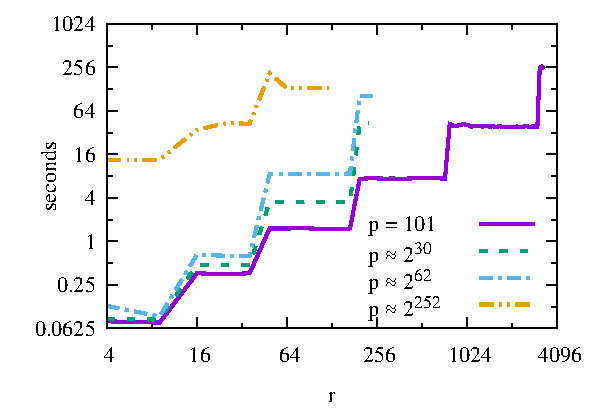
\includegraphics[scale=0.8]{Images/graphe-101-149-269.pdf}
  \end{figure}
\end{frame}

%%%%%%%%%%%%%%%%%%%%%%%%%%%%%%%%%%%%%%%%%%%%%%%%%%%%%%%%%%%% 

\begin{frame}
  \frametitle{Conclusion}
  \orangebox{Contribution}{
    \begin{itemize}
    \item New tools for navigating isogeny volcanoes. 

    \item A faster variant of Couveignes' algorithm.

    \end{itemize}
  }
  \orangebox{Future work}{
    \begin{itemize}
    \item Compare implementation to other algorithms (esp. Lercier-Sirvent).
      % \item Directly generalize to curves not on the crater.
    \item Give an analogous algorithm for Atkin primes.
    \item Analyze our techniques to navigate the volcano in other
      settings: point counting, computation of endomorphism rings, Hilbert
      class polynomials, modular polynomials.
    \end{itemize}}

  % Code available on GitHub: \url{https://github.com/Hugounenq-Cyril/Two_curves_on_a_volcano}
\end{frame}

%%%%%%%%%%%%%%%%%%%%%%%%%%%%%%%%%%%%%%%%%%%%%%%%%%%%%%%%%%%% 

\setbeamertemplate{headline}{\relax}
\setbeamertemplate{footline}{\relax}
\begin{frame}
  \begin{center}
    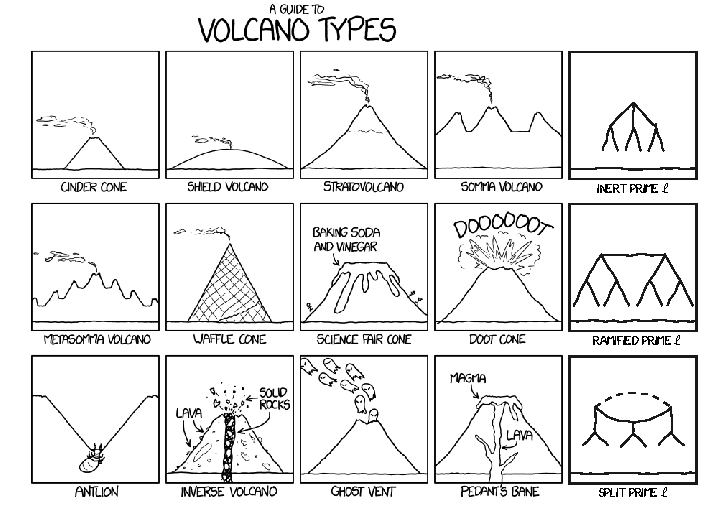
\includegraphics[width=.9\hsize]{Images/volcan}
  \end{center}
  \tiny Modified from  \href{http://xkcd.com/1714/}{xkcd.com/1714}
\end{frame}

\end{document}
